\chapter{Methods}

The aim of this thesis is to use inverse design to find a phononic beamsplitter,
a task that can be divided into three parts: 
First, some definitions of what
should be designed and what constitutes a ``good'' design needs to be made.
Second, we need a way to calculate the gradient of the ``goodness'' with respect
to the design.
And lastly, we need a gradient based optimization algorithm to find the optimal
design.
All of this will be described in this chapter.

\section{Design}

The device design to be optimized can be seen in \cref{fig:bs-design}.
The input and output waveguides consists of unit cells like the one in
\cref{fig:unitcell}.
The values for the parameters in the sketch are given in \cref{tab:params}.
The reason for using this mode in this waveguide is that it has been shown to be
interesting for avoiding mechanical leakage into the substrate on which it is
clamped, as well as retaining a high optomechanical
coupling.\cite{kolvik_clamped_2023}

Inside the design area, there can be one of two kinds of designs.
The first is a \emph{continuous design}, meaning that the material parameters
$\rho$ and $C_{ijkl}$ are continuously varying. The range of values that they
can take are between the density and elasticity of pure silicon and that of air.
Any in-between values are obviously not something that can be physically
realized, but it is useful as a first step in the optimization.
The second kind is a binary design, where each point either has silicon or not
and there are no in-between values.
This is accomplished using level-set methods, which will be explained in
\cref{sec:level-set}.

\begin{figure}[htpb]
	\centering
	\def \a{0.5}
\def \w{1.0}
\def \hx{0.13}
\def \hy{0.3}

\tikzset{
	unitcell/.pic={
		\draw[pic actions] (-0.5*\a, -0.5*\w) rectangle (0.5*\a, 0.5*\w);
		\draw[fill=white] (0, 0) circle [x radius=\hx, y radius=\hy];
	}
}

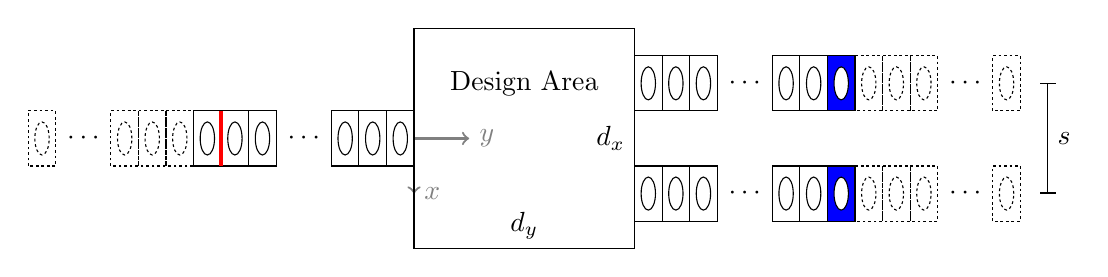
\begin{tikzpicture}[scale=0.7]
	\def \designx{4.0}
	\def \designy{4.0}
	\def \outputh{1.0}
	\def \nunitcells{16}
	\def \nnonpmls{10}

	% Coordinate system
	\draw[gray, thick, ->] (0,0) -- (0,-1) node [anchor=west] {$x$};
	\draw[gray, thick, ->] (0,0) -- (1,0) node [anchor=west] {$y$};

	% Input waveguide
	\path
		(-0.5*\a, 0) pic[transform shape] {unitcell}
		(-1.5*\a, 0) pic[transform shape] {unitcell}
		(-2.5*\a, 0) pic[transform shape] {unitcell}
		(-4.0*\a, 0) node {$\cdots$}
		(-5.5*\a, 0) pic[transform shape] {unitcell}
		(-6.5*\a, 0) pic[transform shape] {unitcell}
		(-7.5*\a, 0) pic[transform shape] {unitcell};
	\draw[red, ultra thick]
		(-7*\a, -0.5*\w) --
		(-7*\a, +0.5*\w);
	\begin{scope}[dash=on 1pt off 1pt phase 0pt]
	\path
		(-8.5*\a, 0) pic[transform shape] {unitcell}
		(-9.5*\a, 0) pic[transform shape] {unitcell}
		(-10.5*\a, 0) pic[transform shape] {unitcell}
		(-12.0*\a, 0) node {$\cdots$}
		(-13.5*\a, 0) pic[transform shape] {unitcell};
	\end{scope}

	% Design area
	\draw (0, -\designx / 2) rectangle (\designy, \designx / 2);
	\node at (\designy / 2, 1) {Design Area};
	\node[left] at (\designy, 0) {$d_x$};
	\node[above] at (\designy/2, -\designx/2) {$d_y$};

	% Output waveguide
	\begin{scope}[xshift=\designy cm, yshift=\outputh cm]
	\path
		(0.5*\a, 0) pic[transform shape] {unitcell}
		(1.5*\a, 0) pic[transform shape] {unitcell}
		(2.5*\a, 0) pic[transform shape] {unitcell}
		(4.0*\a, 0) node {$\cdots$}
		(5.5*\a, 0) pic[transform shape] {unitcell}
		(6.5*\a, 0) pic[transform shape] {unitcell}
		(7.5*\a, 0) pic[transform shape, fill=blue] {unitcell};
	\begin{scope}[dash=on 1pt off 1pt phase 0pt]
	\path
		(8.5*\a, 0) pic[transform shape] {unitcell}
		(9.5*\a, 0) pic[transform shape] {unitcell}
		(10.5*\a, 0) pic[transform shape] {unitcell}
		(12.0*\a, 0) node {$\cdots$}
		(13.5*\a, 0) pic[transform shape] {unitcell};
	\end{scope}
	\end{scope}
	\begin{scope}[xshift=\designy cm, yshift=-\outputh cm]
	\path
		(0.5*\a, 0) pic[transform shape] {unitcell}
		(1.5*\a, 0) pic[transform shape] {unitcell}
		(2.5*\a, 0) pic[transform shape] {unitcell}
		(4.0*\a, 0) node {$\cdots$}
		(5.5*\a, 0) pic[transform shape] {unitcell}
		(6.5*\a, 0) pic[transform shape] {unitcell}
		(7.5*\a, 0) pic[transform shape, fill=blue] {unitcell};
	\begin{scope}[dash=on 1pt off 1pt phase 0pt]
	\path
		(8.5*\a, 0) pic[transform shape] {unitcell}
		(9.5*\a, 0) pic[transform shape] {unitcell}
		(10.5*\a, 0) pic[transform shape] {unitcell}
		(12.0*\a, 0) node {$\cdots$}
		(13.5*\a, 0) pic[transform shape] {unitcell};
	\end{scope}
	\end{scope}
	\draw[|-|]
		(15*\a + \designy, -\outputh) -- node[right] {$s$}
		(15*\a + \designy, \outputh);
		
\end{tikzpicture}

	\caption{
		Device design to be optimized.
		At the red line, a wave traveling right is excited.
		On the blue unit cells is where the output is measured.
		The dashed unit cells are \glspl{pml}
	}
	\label{fig:bs-design}
\end{figure}
\tododec{Are the dx and dy in \cref{fig:bs-design} clear? I thought of having arrows but it
feels like the image gets quite messy then}

\begin{table}[htpb]
	\centering
	\caption{%
		Values for the geometric parameters of the device.
		Reference \cref{fig:bs-design,fig:unitcell} for what the quantities
		mean. The only parameter not mentioned there is $h$, which is the height
		of the structure.
	}%
	\label{tab:params}

	\begin{tabular}{cc}
		\toprule
		Parameter & value\\
		\midrule
		$a$ & \qty{187}{\nm}\\
		$w$ & \qty{187}{\nm}\\
		$h_x$ & \qty{153.5}{\nm}\\
		$h_y$ & \qty{49.5}{\nm}\\
		$h$ & \qty{220}{\nm}\\
		$d_x$ & $6 w$\\
		$d_y$ & $4 w$\\
		$s$ & $3 w$\\
		\bottomrule
	\end{tabular}
\end{table}

\tododec{Write about why we use the mode we use, and why I clamp the bottom. Can
reference Johan and Pauls paper}

\subsection{Perfectly Matched Layers (PMLs)}

Ideally, we would like to have infinite waveguides but that cannot be done in
practice.
Instead, \glspl{pml} are placed at the caps of the input and output waveguides.
The purpose of the \gls{pml} is to absorb any incoming waves without reflection,
which would make it act as if there was an infinite waveguide on the other side
into which the waves propagate indefinitely.
The way to accomplish this is to add an imaginary component to the density of
the material.
If there is an abrupt transition from a real density to a significant imaginary
part, reflections will be created at that transition instead.
Therefore, the imaginary part is taken to be exponentially increasing:
\begin{equation}
	\rho_\text{im} = \rho_\text{si} \cdot s \cdot e^{-\abs{y-y_0} / d}
\end{equation}

\begin{figure}[htpb]
	\centering
	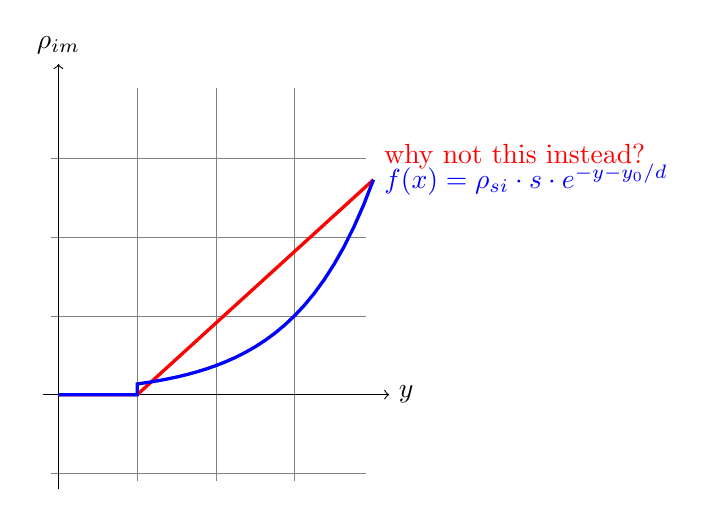
\begin{tikzpicture}[domain=1:4]
		\draw[very thin,color=gray] (-0.1,-1.1) grid (3.9,3.9);

		\draw[->] (-0.2,0) -- (4.2,0) node[right] {$y$};
		\draw[->] (0,-1.2) -- (0,4.2) node[above] {$\rho_\text{im}$};
		\draw[color=red, very thick] (0,0) -- (1,0) -- plot (\x,{(\x-1) *
			0.05*exp(4) / 3})
			node[anchor=south west] {why not this instead?};
		\draw[color=blue, very thick] (0,0) -- (1,0) -- plot (\x,{0.05*exp(\x)})
			node[right] {$f(x) = \rho_\text{si} \cdot s \cdot e^{-\abs{y-y_0} / d}$};
	\end{tikzpicture}
	\caption{Profile of the imaginary component of the waveguides}
	\label{fig:}
\end{figure}

\todoblk{Hold up\ldots why do I choose an exponentially increasing imaginary
	component. If the two possible sources of reflections are the discontinuous
	jump when the pml starts and that the increase is too steep, then why not
	just use a straight line?
}


\subsection{Level-set}\label{sec:level-set}

Ultimately, we want our device to consist of regions of material and regions of
no material.
There are basically two ways of doing this.
The first, and perhaps most intuitive,
is to simply store the coordinates of the boundary between the filled and empty
regions.
In addition to storing the coordinates, one must also store which points
neighbour which.
The second method, which is the one used in this report, is called
the \emph{level-set method}.
In this method, the boundary is not directly stored, but rather is stored via an
\emph{implicit function}, $\phi(x)$, defined such that the boundary is the
0-isocontour of $\phi$.

There are two main advantages of using the level-set method rather than
directly storing the boundary points.
Firstly, when moving the boundary we would like to do so in the normal
direction, as moving it along itself has no effect.
Computing the normal direction of a directly stored boundary is slightly cumbersome,
though certainly achievable.
With level-set, moving the boundary in the normal direction is as easy as adding
a constant to the implicit function.
Secondly, while the boundary is changing the resolution in one part might need
to be increased while the resolution in another needs to be decreased. Deciding
where and when to add new points is non-trivial when directly storing the
boundary. Furthermore, if two boundaries merge, or if one splits in two, points
need to be removed and the connectivities changed, which is quite complex.
\Cref{fig:direct_troubles} illustrates these problems with direct storage concretely.
Both of these issues are automatically handled with the level-set method.
\tododec{How? (Isn't it obvious?)}

\begin{figure}[htpb]
	\centering
	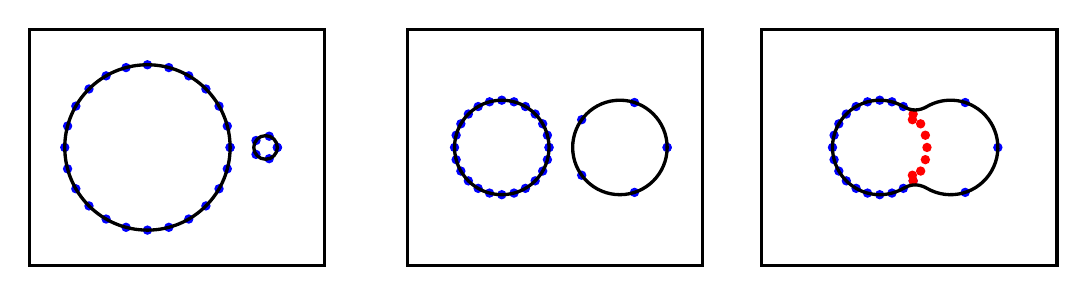
\begin{tikzpicture}[scale=1.5, very thick]
	\coordinate (ca) at (0,0);
	\coordinate (cb) at (1,0);
	\def\radiusa{0.7cm}
	\def\radiusb{0.1cm}
	\def\radpt{0.7pt}
	\draw (-1,-1) rectangle (1.5,1);
	\foreach \i in {0,15,...,360}{% 
		\filldraw [blue]  (ca)++(\i:\radiusa) circle (\radpt);
	}
	\foreach \i in {0,72,...,360}{% 
		\filldraw [blue]  (cb)++(\i:\radiusb) circle (\radpt);
	}
	\draw (ca) circle[radius=\radiusa];
	\draw (cb) circle[radius=\radiusb];

	\begin{scope}[xshift=3cm]
		\coordinate (ca) at (0,0);
		\coordinate (cb) at (1,0);
		\def\radiusa{0.4cm}
		\def\radiusb{0.4cm}
		\draw (-0.8,-1) rectangle (1.7,1);
		\foreach \i in {0,15,...,360}{% 
			\filldraw [blue]  (ca)++(\i:\radiusa) circle (\radpt);
		}
		\foreach \i in {0,72,...,360}{% 
			\filldraw [blue]  (cb)++(\i:\radiusb) circle (\radpt);
		}
		\draw (ca) circle[radius=\radiusa];
		\draw (cb) circle[radius=\radiusb];
	\end{scope}
	\begin{scope}[xshift=6cm]
		\coordinate (ca) at (0.2,0);
		\coordinate (cb) at (0.8,0);
		\def\radiusa{0.4cm}
		\def\radiusb{0.4cm}
		\draw (-0.8,-1) rectangle (1.7,1);
		\foreach \i in {60,75,...,315}{% 
			\filldraw [blue]  (ca)++(\i:\radiusa) circle (\radpt);
		}
		\foreach \i in {-72,0,72}{% 
			\filldraw [blue]  (cb)++(\i:\radiusb) circle (\radpt);
		}
		\foreach \i in {-45, -30, ..., 45}{% 
			\filldraw [red]  (ca)++(\i:\radiusa) circle (\radpt);
		}
		\foreach \i in {144, -144}{% 
			\filldraw [red]  (cb)++(\i:\radiusb) circle (\radpt);
		}
		\draw (ca)++(60:\radiusa)
			arc[radius=\radiusa, start angle=60, end angle=300]
			to[out=30, in=150]
			([shift=(240:\radiusb)] cb)
			arc[radius=\radiusb, start angle=240, end angle=480]
			to[out=210, in=-30]
			cycle;
		%\draw (cb) circle[radius=\radiusb];
	\end{scope}
\end{tikzpicture}

	\caption{%
		Possible evolution of boundary. In the leftmost figure, the
		boundary is defined by pretty much evenly spaced points. In the center figure
		the boundaries have moved and the spacing is no longer even, and the
		right circle is very poorly resolved.
		The rightmost figure shows the boundary after the two circles moved
		closer together. Now there are multiple points that need to be removed,
		marked in red, and the connectivity of the points that remain must be
		changed such that the two boundaries are merged.
	}
	\label{fig:direct_troubles}
\end{figure}

There are of course a lot of possible functions $\phi(x)$ that have a given
boundary as it's 0-isocontour.
There is one choice that simplifies a lot of calculations though: the signed
distance function.
This function is defined as the distance from the closest point on the boundary,
with a plus sign if it is inside and a minus sign if it is outside the boundary.
It has the advantage that if one wishes to locally shift the boundary some
length $s$ in the normal direction, then simply add $s$ to the function there.
\Cref{fig:add_shift} shows this effect in one dimension.
\todowrt{
	Create another figure that shows it in two dimensions.
	I'm thinking a circular boundary, and adding $s$ in the left half and
	subtracting $s$ in the right half. Alternatively adding $s\cdot x$ (unit circle
	centered on 0) so that it will be smooth
}

\begin{figure}[htpb]
	\centering
	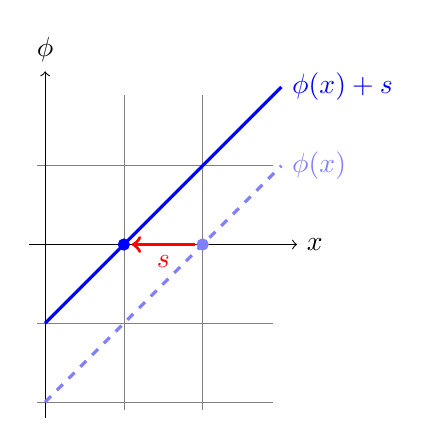
\begin{tikzpicture}[domain=0:3]
		\draw[very thin,color=gray] (-0.1,-2.1) grid (2.9,1.9);

		\draw[->] (-0.2,0) -- (3.2,0) node[right] {$x$};
		\draw[->] (0,-2.2) -- (0,2.2) node[above] {$\phi$};
		\draw[color=blue!50, dashed, very thick] plot (\x,{\x-2})
			node[right] {$\phi(x)$};
		\draw[color=blue, very thick] plot (\x,{\x-1})
			node[right] {$\phi(x)+s$};
		\filldraw[color=blue!50] (2,0) circle[radius=2pt];
		\filldraw[color=blue]    (1,0) circle[radius=2pt];
		\draw[color=red, ->, very thick] (1.9,0) --
			node[below] {$s$}
			(1.1,0);
	\end{tikzpicture}
	\caption{Adding $s$ to the signed distance function shifts boundary by $s$.}
	\label{fig:add_shift}
\end{figure}

\tododec{Write about how I use it? This feels like it should come after I've
talked about computing the derivative.}

\subsection{Objective function}

\tododec{Maybe I'll only mention that $f$ is an integral of the displacement
	field in the theory and here give the specific formula:
}
\begin{equation}
	\fobj = \int_{\Omega_1} \vec{m_1}^*(\vec{x}) \vec{u}(\vec{x})
	\dl{x} + \int_{\Omega_2} \vec{m_2}^*(\vec{x}) \vec{u}(\vec{x})
\end{equation}

\tododec{Paragraph about pure part of objective function, enforcing the minimum
feature size}

\section{Adjoint Simulation}

\tododec{Give the explicit formula for the gradient now that the objective
function has been fully defined}

\section{Optimization}

\tododec{Describe what optimization algorithm was used, as well as how this
	changed during the simulation. E.g.\ first 200 iterations ADAM; next ADAM
	but with sigmoid function application; sigmoid + feature size; and finally level-set.
}
